\documentclass[openany,g5paper,electronic]{kthesis}

\setcounter{tocdepth}{4}
\setcounter{secnumdepth}{4}

\usepackage[T1]{fontenc}
\usepackage{textcomp}
\usepackage{lmodern}
\usepackage[latin1,utf8]{inputenc}
\usepackage[swedish, english]{babel}
\usepackage{tocloft}
\usepackage{multirow}
\usepackage{adjustbox}
\usepackage{graphicx,booktabs}
\usepackage{float}
\usepackage{rotating}
\usepackage{amsthm}
\usepackage{adjustbox}
\usepackage{varwidth} %for the varwidth minipage environment
\usepackage[listings,skins]{tcolorbox}
\usepackage{csquotes}
\usepackage{makeidx} 
\usepackage{enumitem}
%\usepackage{graphics}
%\usepackage{amssymb}
%\usepackage{amsmath}
\usepackage{graphicx}
\usepackage{caption}
\usepackage{listings}
\usepackage{newfloat}
\usepackage[cmex10]{amsmath}
\usepackage{subcaption}
\usepackage[square,numbers]{natbib}
%\usepackage{color} 
%\usepackage{transparent} 
%\usepackage{bm} % bold math
%\usepackage{fmtcount}
%\usepackage{booktabs}
\usepackage{xspace}
\usepackage{tikz}
%\usepackage{algpseudocode}
%\usepackage{algorithm}
\usepackage{algorithm2e}
\usepackage{url}
\usepackage{xurl}
%\usepackage{cite}
\PassOptionsToPackage{hyphens}{url}\usepackage{hyperref}
\usepackage[singlelinecheck=off]{caption}
\hypersetup{
    colorlinks,
    citecolor=black,
    filecolor=black,
    linkcolor=black,
    urlcolor=black
}

% FONTS
\usepackage{lmodern}
\usepackage[T1]{fontenc}
\usepackage{xifthen}% provides \isempty test
\usepackage{xcolor}
\usepackage[explicit]{titlesec}
\usepackage{titletoc}
\usepackage{pdfpages}
\usepackage{comment}
\usepackage[
    left = \flqq{},% 
    right = \frqq{},% 
    leftsub = \flq{},% 
    rightsub = \frq{} %
]{dirtytalk}

% Layout
\definecolor{bluekth}{rgb}{0.16, 0.42, 0.705}

% 0.16, 0.42, 0.705  107/255


% chapter tiltes formatting
\titleformat{\chapter}[display]
  {\LARGE}
  {\renewcommand{\thechapter}{{\color{gray}0}\arabic{chapter}\color{gray}\vspace{2.0ex}\titlerule}
  %\colorbox{blacm}
  {{\bfseries\fontsize{40}{50}\selectfont
  \thechapter\hspace*{-1.5cm}
    \parbox[t][1.2cm][t]{1cm}{%
      \centering\textcolor{black}  {}}}}}
  {-3ex}
  {%\color{black}\titlerule
  \vspace{-12.5ex}\filleft\parbox[b]{0.5\textwidth}{\begin{flushright}\MakeUppercase{#1}\\\end{flushright}}\hspace*{-0.08cm}\vspace{-0.5cm}}
  [\vspace{0.1ex}]
% chapter tiltes spacing
\titlespacing*{\chapter}{0pt}{10pt}{50pt}

% section tiltes formatting
\titleformat{\section}
  {\LARGE}{\MySecSquare\ \thesection}{1em}{#1}

\titleformat{name=\section,numberless}
  {\Large}{\MySecSquare}{1em}{#1}

% subsection tiltes formatting
\titleformat{\subsection}
  {\large}{\MySecSquare}{1em}{#1}

\titleformat{name=\subsection,numberless}
  {\large}{\hspace{0.25em}\MySecSquare\hspace{0.45em}\thesubsection}{1em}{#1}



% formatting for chapter entries in ToC  
%\titlecontents{chapter}
%  [1em]{}
%  {\tiny\thecontentslabel{2.3em}}
%  {\hspace*{-2.3em}}
%  {\hfill\contentspage}
  

% formatting for section entries in ToC  
\titlecontents{section}
  [3.0em]
  {\addvspace{3pt}}%
  {\normalsize\contentslabel{2.3em}}
  {}
  {\titlerule*[1pc]{.}\contentspage}


%\titlecontents{subsection}
%  [10.0em]
%  {\addvspace{3pt}}
%  {\normalsize\contentslabel{2.3em}}
%  {\hspace*{-2.3em}}
%  {\titlerule*[1pc]{.}\contentspage}


  
% Square to be used in itemize
\newcommand\MySquare{%
  \leavevmode\hbox to 1.2ex{\hss\vrule height .9ex width .7ex depth -.2ex\hss}}
% Square to be used in section titles
\newcommand\MySecSquare{%
  \leavevmode\hbox to 1.2ex{\hss\vrule height 1.3ex width 1.1ex depth -.2ex\hss}}


% First level of itemize uses a square
\renewcommand\labelitemi{\MySquare}

%\setcounter{tocdepth}{2}
%\setcounter{secnumdepth}{4}

%%% This is a patch for the correct numbering
\newcounter{patchino}


\newcommand{\msubsection}[1]{
  \stepcounter{patchino}
  \setcounter{subsection}{\thepatchino}
  \subsection{#1}
}


\newcommand{\msection}[1]{
  \setcounter{patchino}{0}
  \section{#1}
}

\usetikzlibrary{tikzmark,calc,decorations.pathreplacing}
\newcommand{\Depth}{2}
\newcommand{\Height}{2}
\newcommand{\Width}{2}

\renewcommand{\labelitemi}{\textcolor{IndianRed3}{\bfseries\textbullet}}


%% For autorefname
\addto\extrasenglish{%
  \renewcommand{\sectionautorefname}{Section}
  \renewcommand{\chapterautorefname}{Chapter}
  \renewcommand{\subsubsectionautorefname}{Subsection}
  \renewcommand{\subsectionautorefname}{Subsection}
}
\DeclareGraphicsExtensions{.pdf,.png,.jpg,.eps}

\DeclareFloatingEnvironment[fileext=frm,placement={tph},name=Listing]{code}
\captionsetup[lstlisting]{singlelinecheck=false, margin=0pt}


\newcommand{\termidx}[2][]{%
    \ifthenelse{\isempty{#1}}%
    {#2} % 
    {#1} %
    \index{#2}
  }
  \newcommand{\ie}{\textit{i.e.,}\xspace}
  \newcommand{\etal}{et al.\xspace}


\newcommand{\subscript}[2]{$#1 _ #2$}

\newcommand{\libsodiumfunctions}{869}
\newcommand{\qrcodefunctions}{1849}
\newcommand{\allmewefunctions}{\libsodiumfunctions + \qrcodefunctions}

% Execute a python script for small calculations
\newcommand{\pypy}[1]{\input{|python3 interpreter.py #1}}
\newcommand{\fromjson}[2]{\input{| jq -r '#2' '#1}}

\newcommand{\corpusrosetta}{Rosetta\xspace}
\newcommand{\corpussodium}{Libsodium\xspace}
\newcommand{\corpusqrcode}{QrCode\xspace}


\newcommand{\DTWStatic}{dt\_static\xspace}
\newcommand{\DTW}{TraceDiff\ }
\newcommand{\crow}{CROW\xspace}
\newcommand{\mewe}{MEWE\xspace}
\newcommand{\wmutate}{wasm-mutate\xspace}


\newcommand{\wasm}{Wasm\xspace}
\newcommand{\Wasm}{WebAssembly\xspace}


\usepackage{catchfile}
\newcommand{\getenv}[2][]{%
  \CatchFileEdef{\temp}{"|kpsewhich --var-value #2"}{\endlinechar=-1}%
  \if\relax\detokenize{#1}\relax\temp\else\let#1\temp\fi}




\newcommand{\wrule}[1]{
  \vspace{3mm}\noindent\textbf{#1}
}


% \renewcommand{\texttt}[1]{\lstinline{#1}}


%% TIkz probes
\newcommand\tikzmarkWS[5]{%
\tikz[remember picture, overlay]{%
        \pgfusepath{use as bounding box}%
        \node[right=#3 mm, fill=white!0, draw=black!40,text width=#5,align =center,outer sep=-0.5pt,inner xsep=1pt, inner ysep=1.5pt, rounded corners=3pt,anchor=north, minimum height=#4 mm, text depth = #4 mm] at (1 mm,2 mm) (#1) {#2};
      %\node[right=#3 mm, align=center, shape=circle,text=black,draw=black, fill=white,inner sep=0.5pt] (#1) {#2};
  }
 }
 

\newcommand\tikzmarkMap[5]{%
\tikz[remember picture, overlay]{%
        \pgfusepath{use as bounding box}%
        \node[right=#3 mm, fill opacity=0, draw opacity=0.5,text width=#5,align =center,outer sep=-0.5pt,inner xsep=1pt, inner ysep=1.5pt, rounded corners=3pt,anchor=north, minimum height=#4 mm, text depth = #4 mm] at (1 mm,2 mm) (#1) {};
      %\node[right=#3 mm, align=center, shape=circle,text=black,draw=black, fill=white,inner sep=0.5pt] (#1) {#2};
  }
 }

\newcommand\tikzmarkJS[4]{%
\tikz[remember picture, overlay]{%
        \pgfusepath{use as bounding box}%
        \node[right=#3 mm, fill=yellow!20,text width=2mm,align =center,outer sep=0pt,inner xsep=1pt, inner ysep=0pt, rounded corners=3pt,anchor=north, minimum height=#4 mm, text depth = #4 mm] at (1 mm,2 mm) (#1) {#2};
      %\node[right=#3 mm, align=center, shape=circle,text=black,draw=black, fill=white,inner sep=0.5pt] (#1) {#2};
  }
 }
 
 \newcommand\tikzmarkPROBE[4]{%
\tikz[remember picture, overlay]{%
        \pgfusepath{use as bounding box}%
        \node[right=#3 mm,text width=2mm,align =center,outer sep=0pt,inner xsep=1pt, inner ysep=0pt, rounded corners=3pt,anchor=north, minimum height=#4 mm, text depth = #4 mm] at (1 mm,2 mm) (#1) {};
      %\node[right=#3 mm, align=center, shape=circle,text=black,draw=black, fill=white,inner sep=0.5pt] (#1) {#2};
  }
 }
  
 \newcommand{\toolcite}[1]{\footnote{\url{#1}}}

 \def\checkmark{\tikz\fill[scale=0.4](0,.35) -- (.25,0) -- (1,.7) -- (.25,.15) -- cycle;} 


\newcommand*\badge[1]{ \colorbox{red}{\color{white}#1}}
\newcommand*\badget[1]{\colorbox{red}{\color{white}#1}}
\newcommand*\badgeg[1]{\colorbox{green}{\color{white}#1}}


\makeatletter
\newenvironment{btHighlight}[1][]
{\begingroup\tikzset{bt@Highlight@par/.style={#1}}\begin{lrbox}{\@tempboxa}}
{\end{lrbox}\bt@HL@box[bt@Highlight@par]{\@tempboxa}\endgroup}


\definecolor{commentgreen}{RGB}{176, 176, 176}
\definecolor{rowcolor}{cmyk}{0,0.87,0.68,0.32}
\definecolor{rowcolor2}{cmyk}{ 20, 0, 37, 34}

\definecolor{eminence}{RGB}{108,48,130}
\definecolor{weborange}{RGB}{255,165,0}
\definecolor{frenchplum}{RGB}{129,20,82}
\definecolor{darkgreen}{RGB}{10, 92, 10}


\definecolor{celadon}{rgb}{0.67, 0.88, 0.69}
%\renewcommand{\blue}{}

\newcommand\btHL[1][]{%
  \begin{btHighlight}[#1]\bgroup\aftergroup\bt@HL@endenv%
}
\def\bt@HL@endenv{%
  \end{btHighlight}%   
  \egroup
}
\newcommand{\bt@HL@box}[2][]{%
  \tikz[#1]{%
    \pgfpathrectangle{\pgfpoint{1pt}{0pt}}{\pgfpoint{\wd #2}{\ht #2}}%
    \pgfusepath{use as bounding box}%
    \node[anchor=base west, fill=orange!30,outer sep=0pt,inner xsep=1pt, inner ysep=0pt, rounded corners=3pt, minimum height=\ht\strutbox+1pt,#1]{\raisebox{1pt}{\strut}\strut\usebox{#2}};
  }%
}
\makeatother

\makeatletter


\lstdefinelanguage{C}{
    otherkeywords={},
    morekeywords=[1]{const, int},
    morekeywords=[2]{0},
    morekeywords=[3]{add,const,mul,shl,get,rem_s,rem_u,ne,tee,sub,set,store},
    morekeywords=[4]{},
    morekeywords=[5]{global, get_global, mut, set_global, export, import,loop, memory, data, get_local,if, block,module, set_local,call,br_if,end, all,call_indirect,local,global,module, func, param, result, type},
    morekeywords=[6]{=,;},
    morekeywords=[7]{(,),[,],.},
    sensitive=false,
    morecomment=[l]{;},
    morecomment=[s]{;}{;},
    morestring=[b]",
    keywordstyle=[1]\color{eminence}\bfseries,
    keywordstyle=[3]\color{frenchplum},
    keywordstyle=[5]\color{darkgreen}\bfseries,
    commentstyle=\color{commentgreen}
}

\lstdefinelanguage{WAT}{
    otherkeywords={},
    morekeywords=[1]{i32,f32,i64,f64},
    morekeywords=[2]{0},
    morekeywords=[3]{add,const,mul,shl,get,rem_s,rem_u,ne,tee,sub,set,store},
    morekeywords=[4]{},
    morekeywords=[5]{global, get_global, mut, set_global, export, import,loop, memory, data, get_local,if, block,module, set_local,call,br_if,end, all,call_indirect,local,global,module, func, param, result, type},
    morekeywords=[6]{=,;},
    morekeywords=[7]{(,),[,],.},
    sensitive=false,
    morecomment=[l]{;},
    morecomment=[s]{;}{;},
    morestring=[b]",
    keywordstyle=[1]\color{eminence}\bfseries,
    keywordstyle=[3]\color{frenchplum},
    keywordstyle=[5]\color{darkgreen}\bfseries,
    commentstyle=\color{commentgreen}
}
\lstdefinelanguage{llvm}{
    morecomment = [l]{;},
    morestring=[b]", 
    sensitive = true,
    morekeywords=[2]{i32,f32,i64,f64},
    morekeywords=[3]{
        define, declare, global, constant,
        internal, external, private,
        linkonce, linkonce_odr, weak, weak_odr, appending,
        common, extern_weak,
        thread_local, dllimport, dllexport,
        hidden, protected, default,
        except, deplibs,
        volatile, fastcc, coldcc, cc, ccc,
        x86_stdcallcc, x86_fastcallcc,
        ptx_kernel, ptx_device,
        signext, zeroext, inreg, sret, nounwind, noreturn,
        nocapture, byval, nest, readnone, readonly, noalias, uwtable,
        inlinehint, noinline, alwaysinline, optsize, ssp, sspreq,
        noredzone, noimplicitfloat, naked, alignstack,
        module, asm, align, tail, to,
        addrspace, section, alias, sideeffect, c, gc,
        target, datalayout, triple,
        blockaddress
    },
    morekeywords=[4]{
        fadd, sub, fsub, mul, fmul,
        sdiv, udiv, fdiv, srem, urem, frem,
        and, or, xor,
        icmp, fcmp,
        eq, ne, ugt, uge, ult, ule, sgt, sge, slt, sle,
        oeq, ogt, oge, olt, ole, one, ord, ueq, ugt, uge,
        ult, ule, une, uno,
        nuw, nsw, exact, inbounds,
        phi, call, select, shl, lshr, ashr, va_arg,
        trunc, zext, sext,
        fptrunc, fpext, fptoui, fptosi, uitofp, sitofp,
        ptrtoint, inttoptr, bitcast,
        ret, br, indirectbr, switch, invoke, unwind, unreachable,
        malloc, alloca, free, load, store, getelementptr,
        extractelement, insertelement, shufflevector,
        extractvalue, insertvalue,
    },
    alsoletter={\%},
    keywordsprefix={\%},% All identifiers starting with '%' will be printed as first order keywords.
    keywordstyle=[1]\bfseries,% As mentioned above, these are the keywords starting with '%', like '%5'
    keywordstyle=[2]\color{eminence}\bfseries,
    keywordstyle=[3]\color{darkgreen}\bfseries,
    keywordstyle=[4]\color{frenchplum},
}
\makeatother

\newcommand{\todo}[1]{%
%\refstepcounter{todo}
\noindent\textbf{\badge{TODO}} {\color{red} #1}
%\addcontentsline{td}{todo}
%{\color{red}\thesection.\thetodo\xspace #1}
}

\newcommand{\done}[1]{%
\noindent\textbf{\badgeg{DONE}} {\color{green}#1}
}
\newcommand{\citationneeded}{
  \badget{[?]}
}

\newcommand*\step[1]{
\noindent\tikz[baseline=(char.base)]{
        \node[shape=circle,text=black,draw=black, fill=white,inner sep=1.2pt] (char) {#1};}}



\newtheorem{definition}{Definition}
\providecommand*{\definitionautorefname}{Definition}
\newtheorem{metric}{Metric}
\providecommand*{\metricautorefname}{Metric}



\newtheorem{property}{Property}
\providecommand*{\propertyautorefname}{Property}

\hyphenation{Web-Assembly}
\hyphenation{super-optimizers}
\hyphenation{super-optimize}

%\addcontentsline{td}{todo}
%{\color{red}\thesection.\thetodo\xspace Citation needed}}


\makeatletter
\lstset{
    %language=C,
    basicstyle=\ttfamily\footnotesize\lst@ifdisplaystyle\scriptsize\fi,
    escapeinside={\%*}{*)},
    captionpos=t
}
\makeatother


\lstdefinestyle{CStyle}{
  %numbers=none,
  stepnumber=1,
  numbersep=10pt,
  tabsize=4,
  showspaces=false,
  showstringspaces=false,
  basicstyle=\scriptsize\ttfamily,
  %moredelim=**[is][{\btHL[fill=black!10]}]{`}{`},
  moredelim=**[is][{\btHL[fill=celadon!40]}]{@}{@}
}

\lstdefinestyle{WATStyle}{
  numbers=left,
  stepnumber=1,
  numbersep=5pt,
  tabsize=4,
  showspaces=false,
  showstringspaces=false,
}

\lstdefinestyle{LLVMStyle}{
  numbers=none,
  stepnumber=0,
  numbersep=10pt,
  tabsize=4,
  showspaces=false,
  showstringspaces=true,
}



\getenv[\NOWIDOW]{NOWIDOW}
\ifthenelse{\equal{\NOWIDOW}{True}}%
    {
      \widowpenalties 1 10000
      \raggedbottom

      \setlength{\parskip}{20pt}

      \titlecontents{chapter}[0pc]
      {\addvspace{15pt}}%
      {\large\bfseries}
      {\large\bfseries}
      {\bfseries\hfill\large}%
      
      \titlecontents{subsection}
      [10.0em]{}
      {\normalsize\contentslabel{3.3em}}
      {\hspace*{-2.3em}}
      {\titlerule*[1pc]{ }}

      \titlecontents{section}
      [10.0em]{}
      {\normalsize\contentslabel{3.3em}}
      {\hspace*{-2.3em}}
      {\titlerule*[1pc]{ }}


      \renewcommand\labelitemi{}


        % section tiltes formatting
        \titleformat{\section}
        {\Large}{}{1em}{#1}
        \titleformat{name=\section,numberless}
        {\Large}{}{1em}{#1}

        % subsection tiltes formatting
        \titleformat{\subsection}
        {\Large}{}{1em}{#1}
        \titleformat{name=\subsection,numberless}
        {\Large}{}{1em}{#1}

        \titleformat{\chapter}[display]
        {\LARGE}
        {\renewcommand{\thechapter}{}
        %\colorbox{blacm}
        {{\bfseries\fontsize{30}{40}\selectfont
        \thechapter
          \parbox[c][1.2cm][c]{1cm}{%
            \centering\textcolor{black}  {}}}}}
        {-1ex}
        {%\color{black}\titlerule
        \vspace{-1.9ex}\filleft\MakeUppercase{#1}}
        [
        ]
    } % 
    {} %

%%%%%%%%%%%%%%%%%%%%%%%%%%%%%%%%%%%%%%%
%%%%%%%%% Document starts here %%%%%%%%
%%%%%%%%%%%%%%%%%%%%%%%%%%%%%%%%%%%%%%%
\begin{document}

%%%%%%%%%%%%%%%%%%%%%%%%%%%%%%%%%%%%%%%%%%
%%%%%% First and second pages %%%%%%%%%%%%
%%%%%%%%%%%%%%%%%%%%%%%%%%%%%%%%%%%%%%%%%%

%\title{Runtime randomization and perturbation for virtual machines.}
\title{ Artificial Software Diversification for WebAssembly }
\subtitle{\textbf{sub-title}}
\author{Javier Cabrera-Arteaga}
\date{date}
\thesistype{Doctoral Thesis}
\imprint{Stockholm, Sweden, 2020}
\examen{Teknologie doktorexamen i elektroteknik}
\disputationsdatum{fredagen den 18 januari 2020 klockan 14.00}
\disputationslokal{Sal F3, Lindstedtsvägen 26, Kungliga Tekniska H\"{o}gskolan, Stockholm}
\publisher{Universitetsservice US AB}
\address{KTH Royal Institute of Technology \\School of Electrical Engineering and Computer Science\\ Division of Fusion Plasma Physics \\ SE-10044 Stockholm\\ Sweden}
\isbn{ISBN 100-}
%\issn{ISSN XXX} % No longer used at KTH
\trita{TRITA-EECS-AVL-2020:4}
\kthlogo{KTHLogo}

\pretolerance=10000
\tolerance=4000 
\emergencystretch=10pt
% Create title page using info above
\maketitle

\frontmatter % Pages i, ii, iii, iv, v etc.
%%%%%%%%%%%%%%%%%%%%%%%%%%%%%%%%%%%
%%%%%%%%%%% ABSTRACT %%%%%%%%%%%%%%
%%%%%%%%%%%%%%%%%%%%%%%%%%%%%%%%%%%
\begin{abstract}
\noindent \lipsum[1]

\end{abstract}

\bigskip \bigskip \bigskip \bigskip \bigskip

\setlength{\leftskip}{0.3 cm} \textbf {Keywords:} Lorem, Ipsum, Dolor, Sit, Amet

%%%%%%%%%%%%%%%%%%%%%%%%%%%%%%%%%%%%%%%%
%%%%%%%% SWEDISH ABSTRACT %%%%%%%%%%%%%%
%%%%%%%%%%%%%%%%%%%%%%%%%%%%%%%%%%%%%%%%
\newpage
\selectlanguage{swedish}
\begin{abstract}
\noindent \lipsum[1]
\end{abstract}
\selectlanguage{english}

%%%%%%%%%%%%%%%%%%%%%%%%%%%%%%%%%%%%%%%
%%%%%%% List of papers %%%%%%%%%%%%%%%%
%%%%%%%%%%%%%%%%%%%%%%%%%%%%%%%%%%%%%%%
\chapter{List of Papers}

\let\thefootnote\relax\footnote{Paper I and III are published under license in \textit{Journal of X}}
\begin{enumerate}[I]
	\item \textbf{\textit{Title of paper}} \\
		\textbf{First author}, Second author \\
		\textit{Journal (year)}
\end{enumerate}

%%%%%%%%%%%%%%%%%%%%%%%% Papers NOT included in THESIS
Other contributions by the author not included in the thesis.
\begin{enumerate}[I]
	\setcounter{enumi}{1}
	\item \textbf{\textit{Title of paper}} \\
		\textbf{First author}, Second author \\
		\textit{Journal (year)}
\end{enumerate}
%%%%%%%%%%%%%%%%%%%%%%%%%%%%%%%%%%%%%%%
%%%%%%%% ACKNOWLEDGMENT %%%%%%%%%%%%%%%
%%%%%%%%%%%%%%%%%%%%%%%%%%%%%%%%%%%%%%%
\chapter{Acknowledgement}
\noindent \lipsum[1]

%%%%%%%%%%%%%%%%%%%%%%%%%%%%%%%%
%%%%%%%% ACRONYMS %%%%%%%%%%%%%%
%%%%%%%%%%%%%%%%%%%%%%%%%%%%%%%%
\chapter{Acronyms}
List of commonly used acronyms: \\

\begin{tabular}{llll}
\textbf{AE}		&	Acronym examples \\

\end{tabular}

%\input{Content/Dedication}\clearpage

\mainmatter % Pages 1, 2, 3...
%%%%%%%%%%%%%%%%%%%%%%%%%%%%%%%%%%%%%%
%%%%%% TABLE OF CONTENTS %%%%%%%%%%%%%
%%%%%%%%%%%%%%%%%%%%%%%%%%%%%%%%%%%%%%
\tableofcontents

%%%%%%%%%%%%%%%%%%%%%%%%%%%%%%%%%%%%%%%%%%%%%%%%%%%%%%
%%%%%%%%%%%%% CHAPTER 1: INTRODUCTION %%%%%%%%%%%%%%%%
%%%%%%%%%%%%%%%%%%%%%%%%%%%%%%%%%%%%%%%%%%%%%%%%%%%%%%
\chapter{Energy needs - an introduction}
\label{Intro}
Here is an example for referencing figure \ref{EnergySources}. Example of citing \cite{BP2019} and \cite{Chen2016}.
%%%%%%%%%%%%%% Figure: Energy sources
\begin{figure}[h]
	\centering
	% \includegraphics[scale=0.6]{Figs/Ch1_EnergySources.png}
	\caption{The world's energy consumption by fuel in 2017. }
	\label{EnergySources}
\end{figure}

%%%%%%%%%%%%%%%%%%%%%%%%%%%%%%%%%%%%%%%%
\section{Section}
Example of a table
%%%%%%%%%%%%%%%%%%%%%%%%%%%%%%%% Table: Tokamaks
\begin{table}[t!]
	\centering
	\caption{List of experimental tokamaks worldwide. Note: ITER is currently under construction and the first plasma is predicted for 2025-2028.}
		\begin{tabular}{ccccc}
			\hline
			\textbf{Name} & \textbf{Location} & \textbf{B-field} & \textbf{Major/minor radius}  \\
			\hline
			JET     & England      & 4.0 T & 3.0 m / 1.3 m \\
			ITER    & France       & 5.3 T & 6.2 m / 2.0 m \\
			AUG		& Germany      & 3.1 T & 1.7 m / 0.7 m \\
			WEST	& France	   & 3.7 T & 2.5 m / 0.5 m \\
			TCV     & Switzerland  & 1.5 T & 0.9 m / 0.3 m \\
			DIII-D  & USA          & 2.2 T & 1.7 m / 0.7 m \\
			TFTR 	& USA          & 6.0 T & 2.5 m / 0.9 m \\
			JT-60   & Japan        & 4.0 T & 3.4 m / 1.0 m \\
			K-STAR  & South Korea  & 3.5 T & 1.8 m / 0.5 m \\
			EAST    & China        & 3.5 T & 1.9 m / 0.5 m \\
			\hline
		\end{tabular}
	\label{TokamakTable}
\end{table}


\chapter{Chapter 2}
\label{Ch2label}
\noindent \lipsum[1]

%%%%%%%%%%%%%%%%%%%%%%%%%%%%%%%%%%%%%%%%%%%%%%%%%%%%%%%%%%%%%%%%%%%%%%%%
%%%%%%%%%%%%%%%%%%%%%%%%%%%%%%%%%%%%%%%%%%%%%%%%%%%%%%%%%%%%%%%%%%%%%%%%
%%%%%%%%%%%%%%% CHAPTER 6: Summary of the publications %%%%%%%%%%%%%%%%%
%%%%%%%%%%%%%%%%%%%%%%%%%%%%%%%%%%%%%%%%%%%%%%%%%%%%%%%%%%%%%%%%%%%%%%%%
%%%%%%%%%%%%%%%%%%%%%%%%%%%%%%%%%%%%%%%%%%%%%%%%%%%%%%%%%%%%%%%%%%%%%%%%
\chapter{Summary of the included papers}
\label{Summary}
\noindent \lipsum[1]

%%%%%%%%%%%%%%%%%%%%%%%%%%%%%%%
\section{Paper I - ...}

%%%%%%%%%%%%%%%%%%%%%%%%%%%%%%%%%%%%%%%%%%%%%%%%%%%%%%%%%
%%%%%%%%%%%%%%%%%%%%%%%%%%%%%%%%%%%%%%%%%%%%%%%%%%%%%%%%%
%%%%%%%%%%%% CHAPTER 7: Conclusions %%%%%%%%%%%%%%%%%%%%%
%%%%%%%%%%%%%%%%%%%%%%%%%%%%%%%%%%%%%%%%%%%%%%%%%%%%%%%%%
%%%%%%%%%%%%%%%%%%%%%%%%%%%%%%%%%%%%%%%%%%%%%%%%%%%%%%%%%
\chapter{Conclusions}
\label{Conclusions}
\noindent \lipsum[1]
%%%%%%%%%%%%%%%%%%%%%%%%%%%%%%%

%%%%%%%%%%%%%%%%%%%%%%%%%%%%%%%%%%%%%%%%%%%%%%%
\section{Conclusions}
\noindent \lipsum[1]

%%%%%%%%%%%%%%%%%%%%%%%%%%%%%%%%%%%%%%%%%%%%%%%%%%%%%%%%%
%%%%%%%%%%%%%%%%%%%%%%%%%%%%%%%%%%%%%%%%%%%%%%%%%%%%%%%%%
%%%%%%%%%%%% CHAPTER 8: Personal reflections %%%%%%%%%%%%
%%%%%%%%%%%%%%%%%%%%%%%%%%%%%%%%%%%%%%%%%%%%%%%%%%%%%%%%%
%%%%%%%%%%%%%%%%%%%%%%%%%%%%%%%%%%%%%%%%%%%%%%%%%%%%%%%%%
\chapter{Personal reflections}
\label{PersonalReflections}
\noindent \lipsum[1]

%------------------------------------------------
% CREATING THE BIBLIOGRAPHY
%------------------------------------------------
\bibliographystyle{ieeetr}
\renewcommand{\bibname}{References}% changes default name Bibliography to References
\bibliography{Kappa} % References file

%--------------------------------------------------
%\addcontentsline{toc}{chapter}{Appended papers} % for template purposes
\part{Included papers}
\stepcounter{page} % Skip the current page

% Each chapter is a paper
% chapter tiltes formatting
\titleformat{\chapter}[display]
  {\Large}
  {\renewcommand{\thechapter}{{\color{gray}P}\arabic{chapter}}\hspace*{0.5em}
  %\colorbox{blacm}
  {}}
  {-1ex}
  {%\color{black}\titlerule
  \vspace{-0.5cm}\huge\MakeUppercase{#1}}
  [\vspace{.0ex}
  \color{black}
  \titlerule
  ]
% chapter tiltes spacing
\titlespacing*{\chapter}{0pt}{20pt}{80pt}

\renewcommand{\thechapter}{}\hspace*{-1em}
  %\colorbox{blacm}
  {}
  \titlecontents{chapter}
  [-3.9pc]
  {{\addvspace{8pt}}}%
  {\normalsize}
  {\normalsize}
  {\hfill\large\contentspage}%

% \setcounter{chapter}{0}
\getenv[\ADDCONTRIB]{ADDCONTRIB}

\chapter{WebAssembly Diversification for Malware Evasion}

\textbf{Javier Cabrera-Arteaga}, Tim Toady, Martin Monperrus, Benoit Baudry\\
\emph{Computers \& Security, Volume 131, 2023}\\\\
\url{https://www.sciencedirect.com/science/article/pii/S0167404823002067}\\\\

\ifthenelse{\equal{\ADDCONTRIB}{True}}%
    {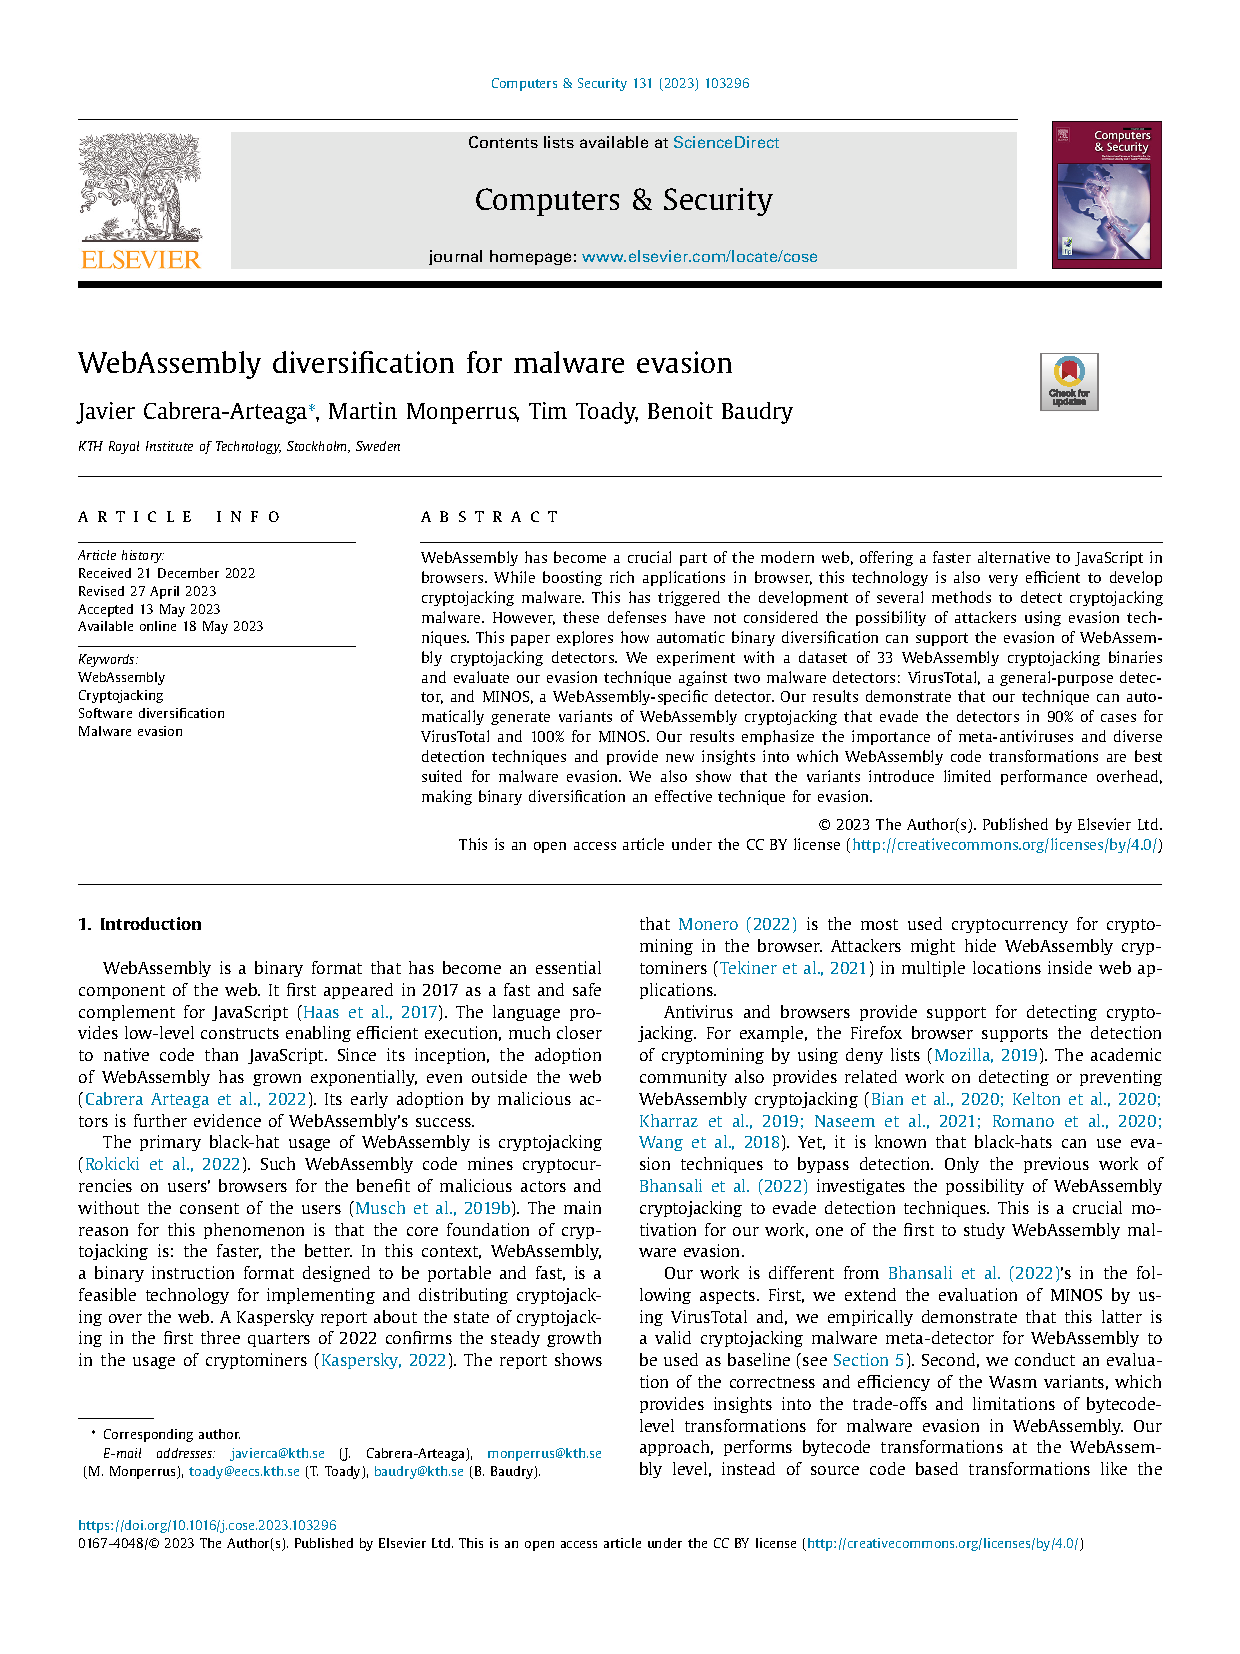
\includepdf[pages=1-16]{papers/evasion.pdf}} % 
    {} %
    

\chapter{\mbox{WASM-MUTATE}:~Fast~and~Effective~Binary~Diversification~for~\mbox{WebAssembly}}
\textbf{Javier Cabrera-Arteaga}, Nick Fitzgerald, Martin Monperrus, Benoit Baudry\\
\emph{Computers \& Security, 2024}\\\\
\url{https://www.sciencedirect.com/science/article/pii/S0167404824000324}\\\\

\ifthenelse{\equal{\ADDCONTRIB}{True}}%
    {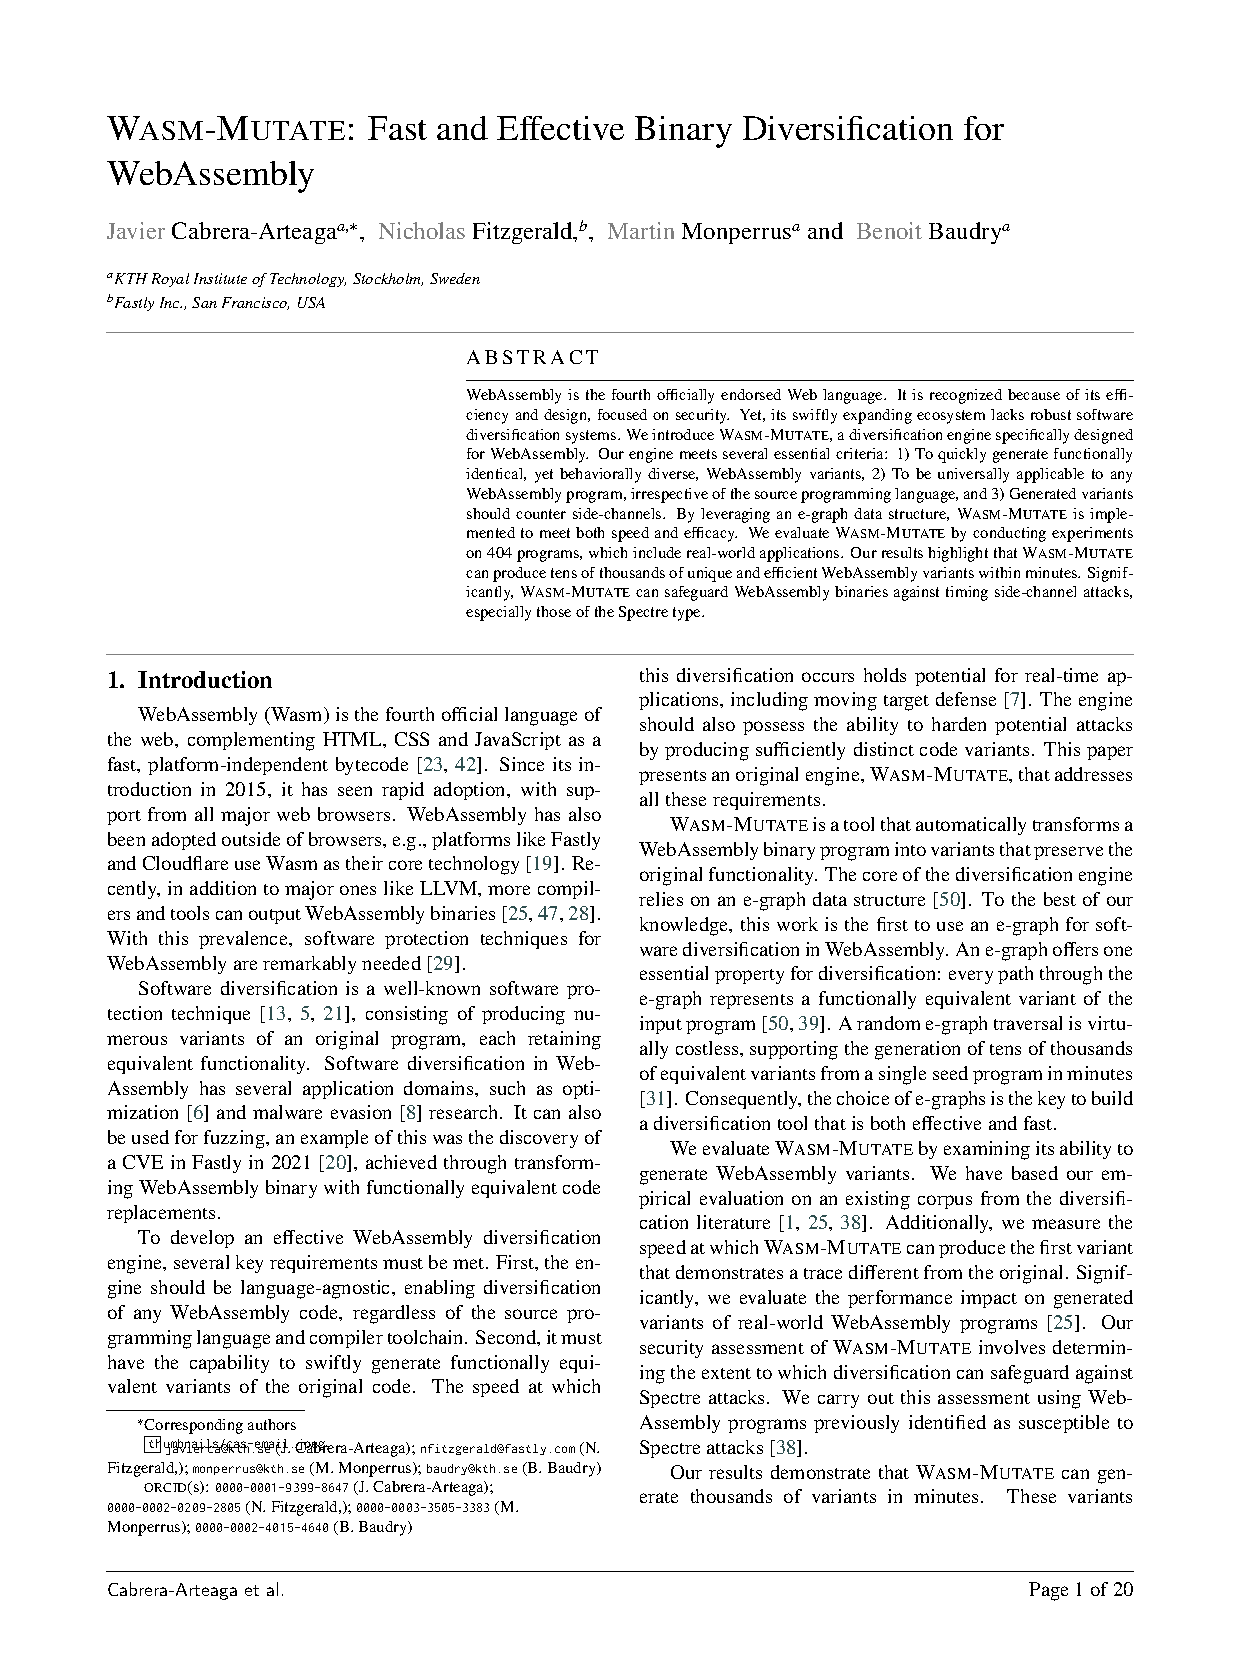
\includepdf[pages=1-20]{papers/wasm-mutate-v2.pdf}} % 
    {} %


% Add paper here
\chapter{CROW: Code Diversification for WebAssembly}

\textbf{Javier Cabrera-Arteaga}, Orestis Floros, Oscar Vera-Pérez, Benoit Baudry, Martin Monperrus\\
\emph{Network and Distributed System Security Symposium (NDSS 2021), Workshop on Measurements, Attacks, and Defenses for the Web}\\\\
\url{https://doi.org/10.14722/madweb.2021.23004}\\

\ifthenelse{\equal{\ADDCONTRIB}{True}}%
    {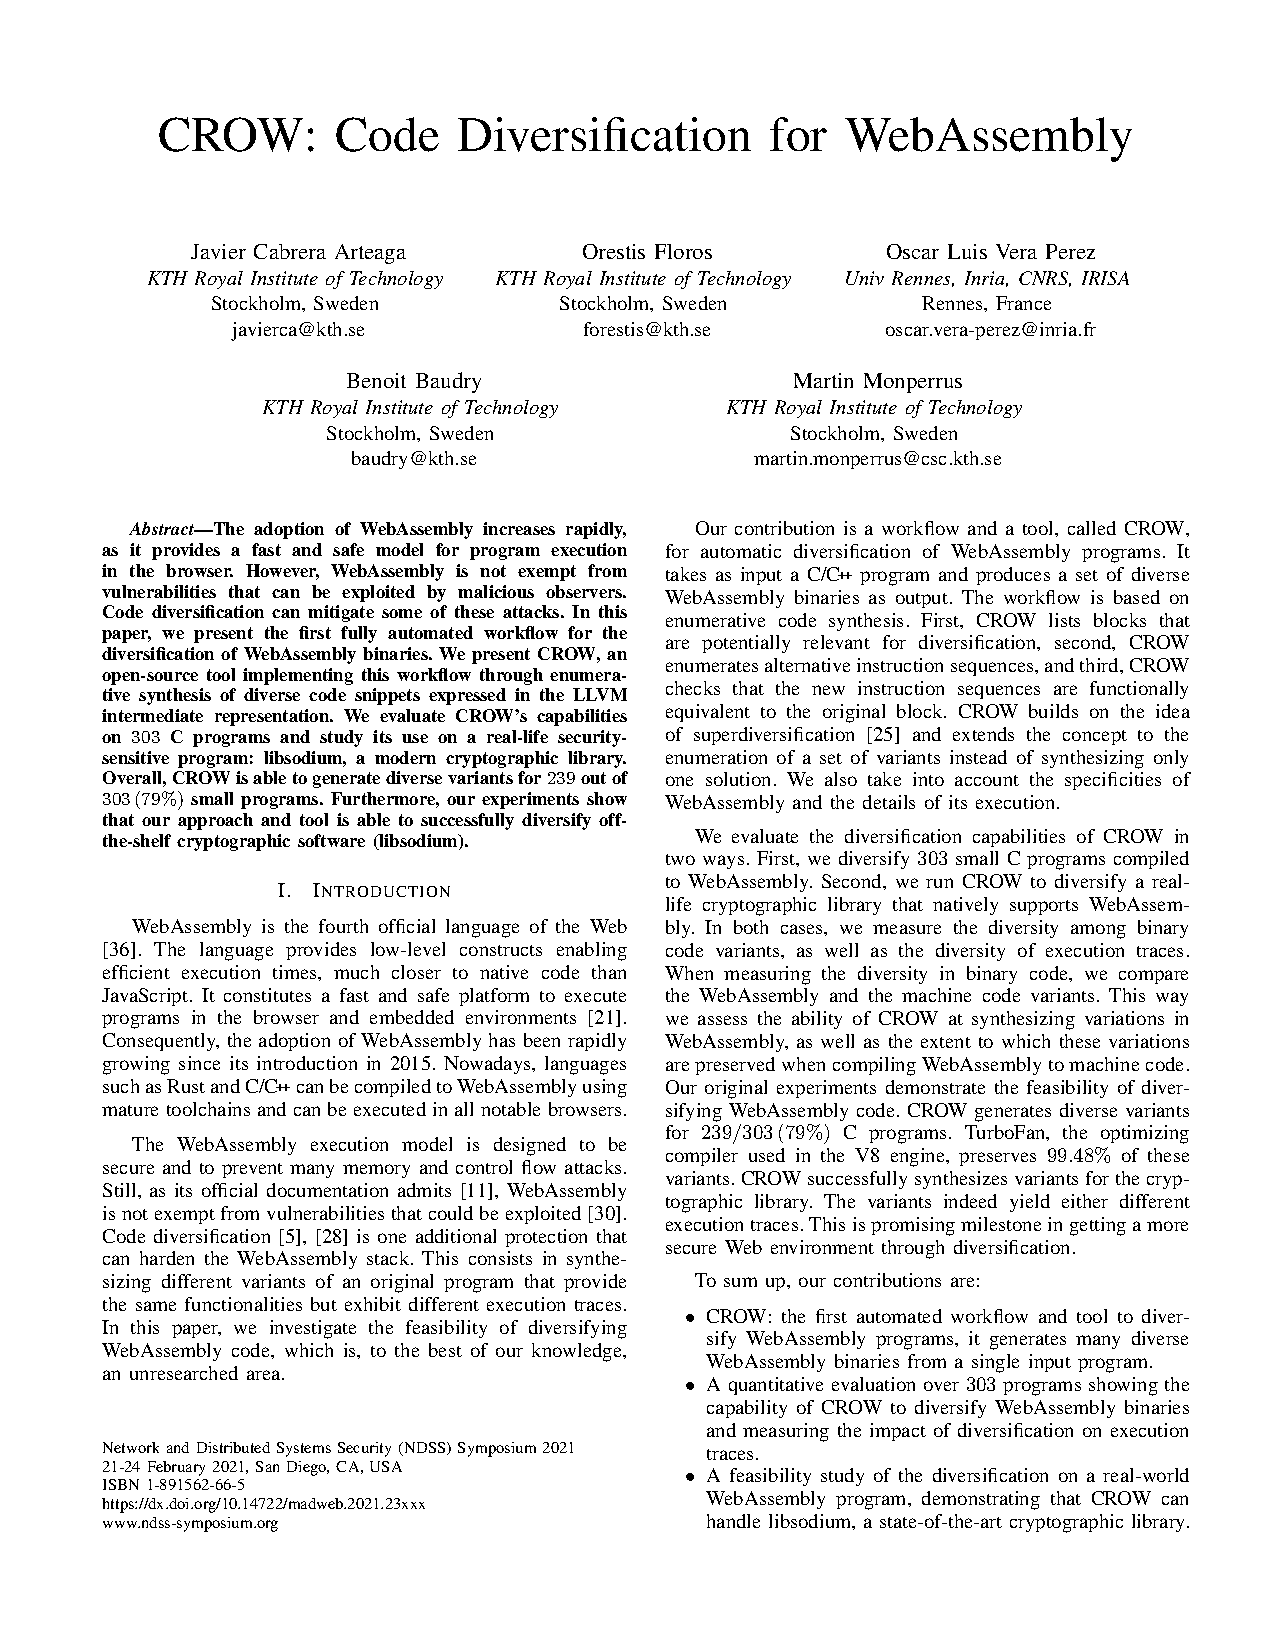
\includepdf[pages=1-12]{papers/crow.pdf}} %
    {} % 
    
\chapter{Multi-Variant Execution at the Edge}

\textbf{Javier Cabrera-Arteaga}, Pierre Laperdrix, Martin Monperrus, Benoit Baudry\\
\emph{Conference on Computer and Communications Security (CCS 2022), Workshop on Moving Target Defense (MTD)}\\\\
 \url{https://dl.acm.org/doi/abs/10.1145/3560828.3564007}\\\\

\ifthenelse{\equal{\ADDCONTRIB}{True}}%
    {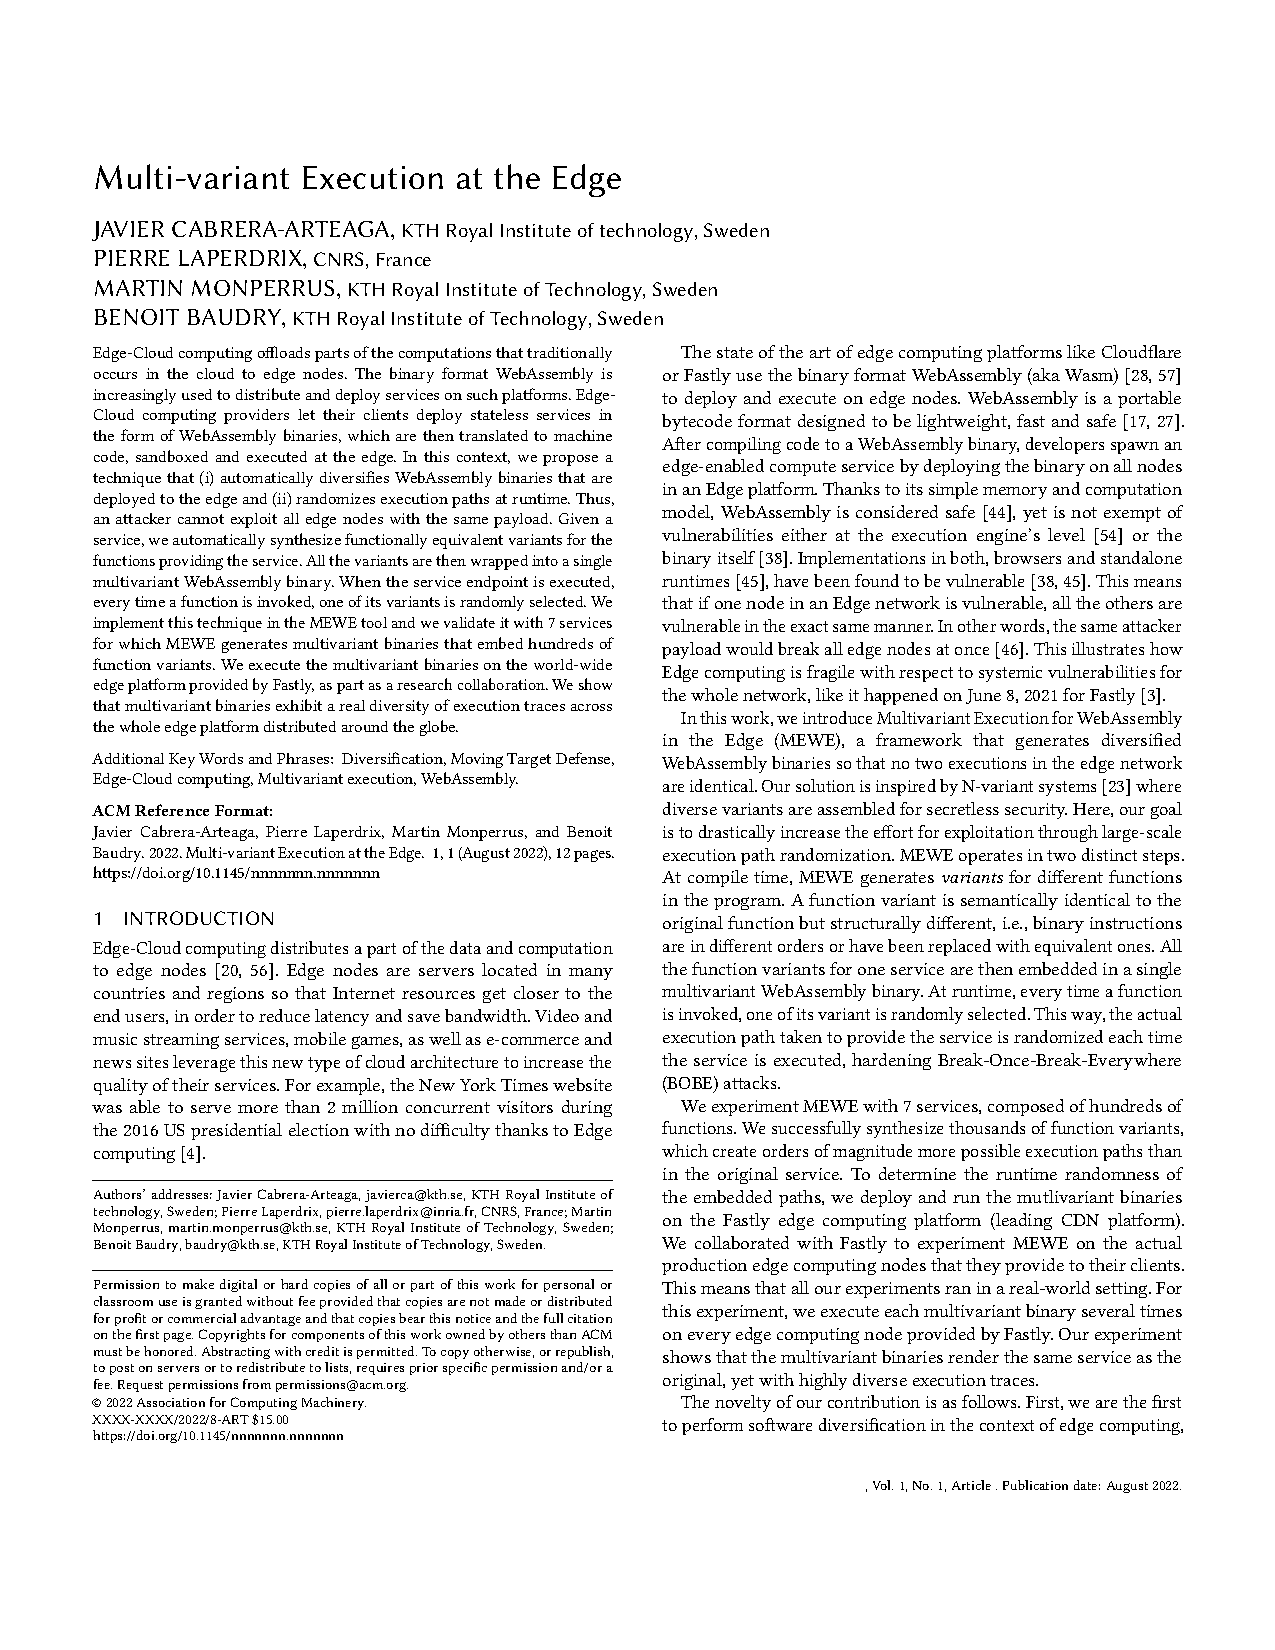
\includepdf[pages=1-12]{papers/mewe_final.pdf}} % 
    {} %
    
  \chapter{Superoptimization of WebAssembly Bytecode}

  \textbf{Javier Cabrera-Arteaga}, Shrinish Donde, Jian Gu, Orestis Floros, Lucas Satabin, Benoit Baudry, Martin Monperrus\\
  \emph{Conference Companion of the 4th International Conference on Art, Science, and Engineering of Programming (Programming 2021), MoreVMs}\\\\
  \url{https://doi.org/10.1145/3397537.3397567}\\
  
  % Add Abstract
  
  \ifthenelse{\equal{\ADDCONTRIB}{True}}%
      {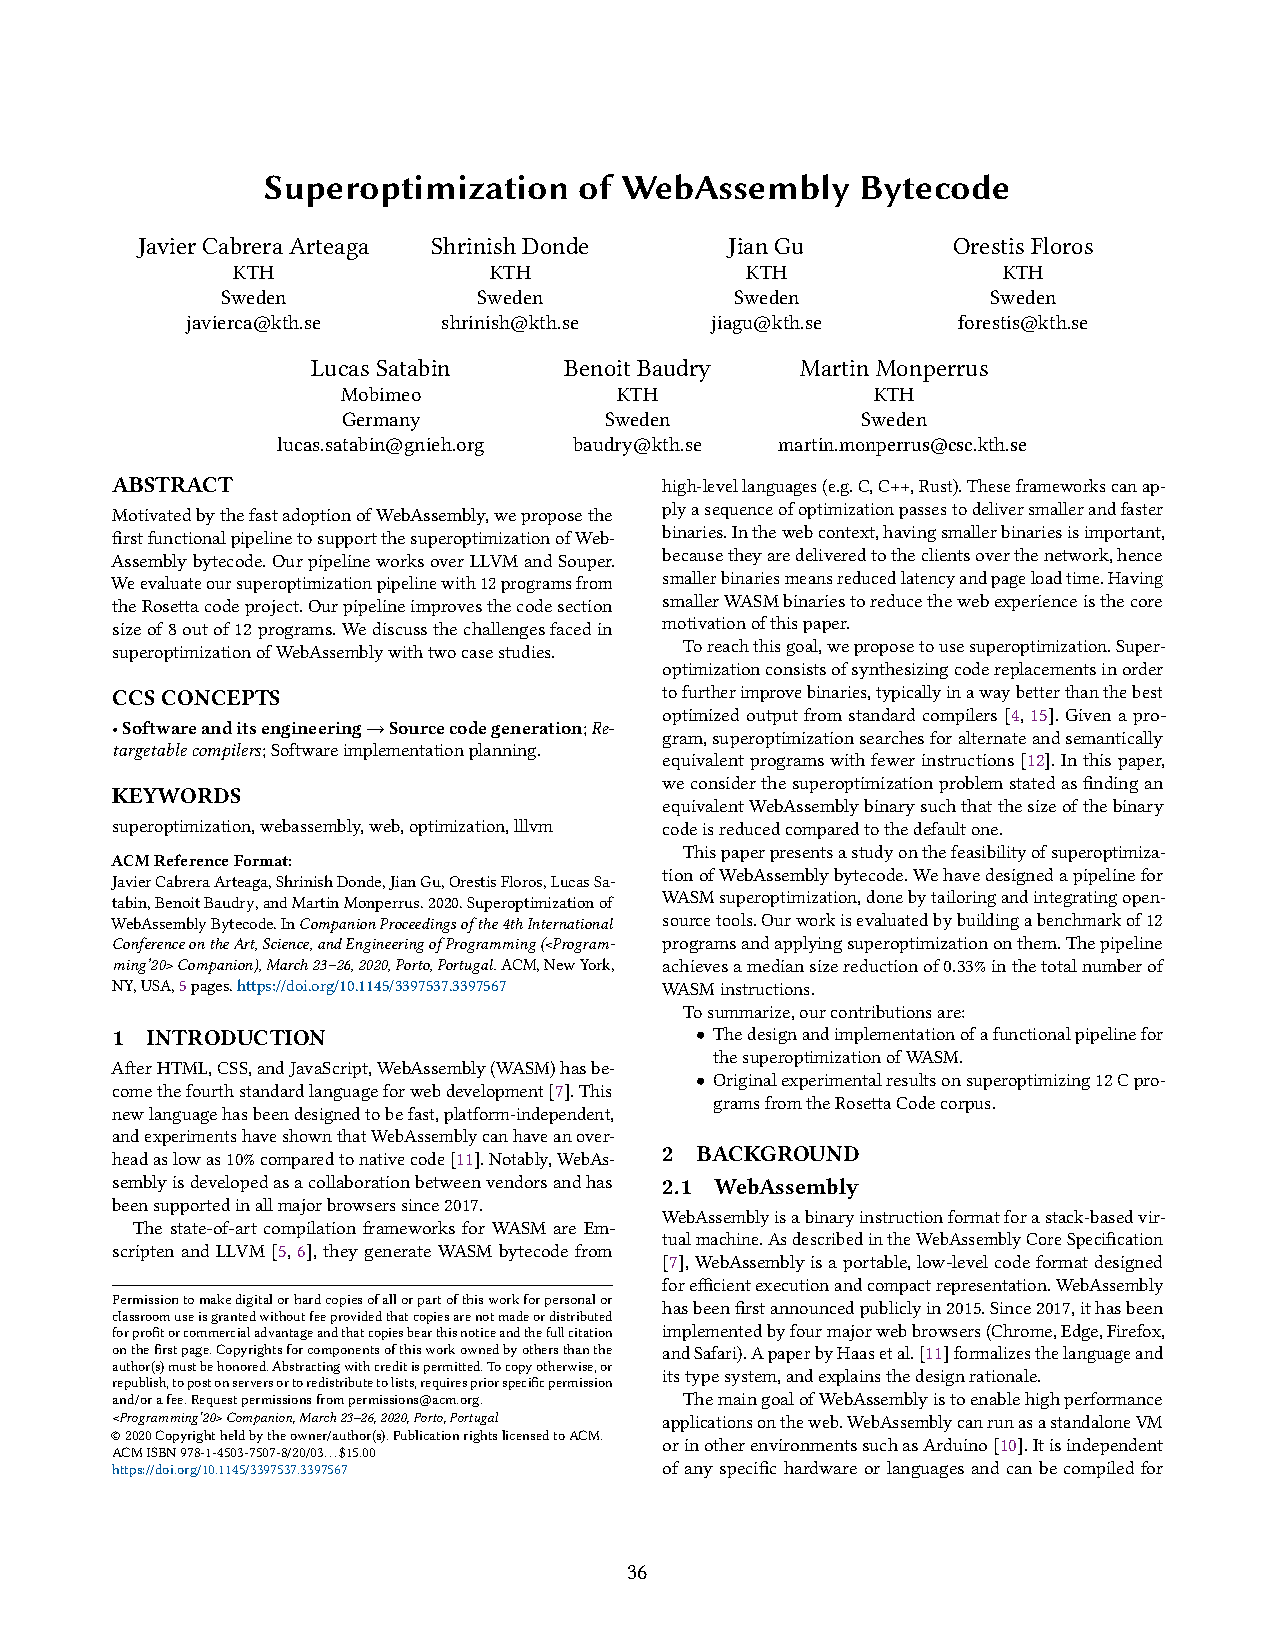
\includepdf[pages=1-5]{papers/souper.pdf}} % 
      {} %
    
\chapter{Scalable Comparison of JavaScript V8 Bytecode Traces}

\textbf{Javier Cabrera-Arteaga}, Martin Monperrus, Benoit Baudry\\
\emph{11th ACM SIGPLAN International Workshop on Virtual Machines and Intermediate Languages (SPLASH 2019)}\\\\
\url{https://doi.org/10.1145/3358504.3361228}\\


\ifthenelse{\equal{\ADDCONTRIB}{True}}%
    {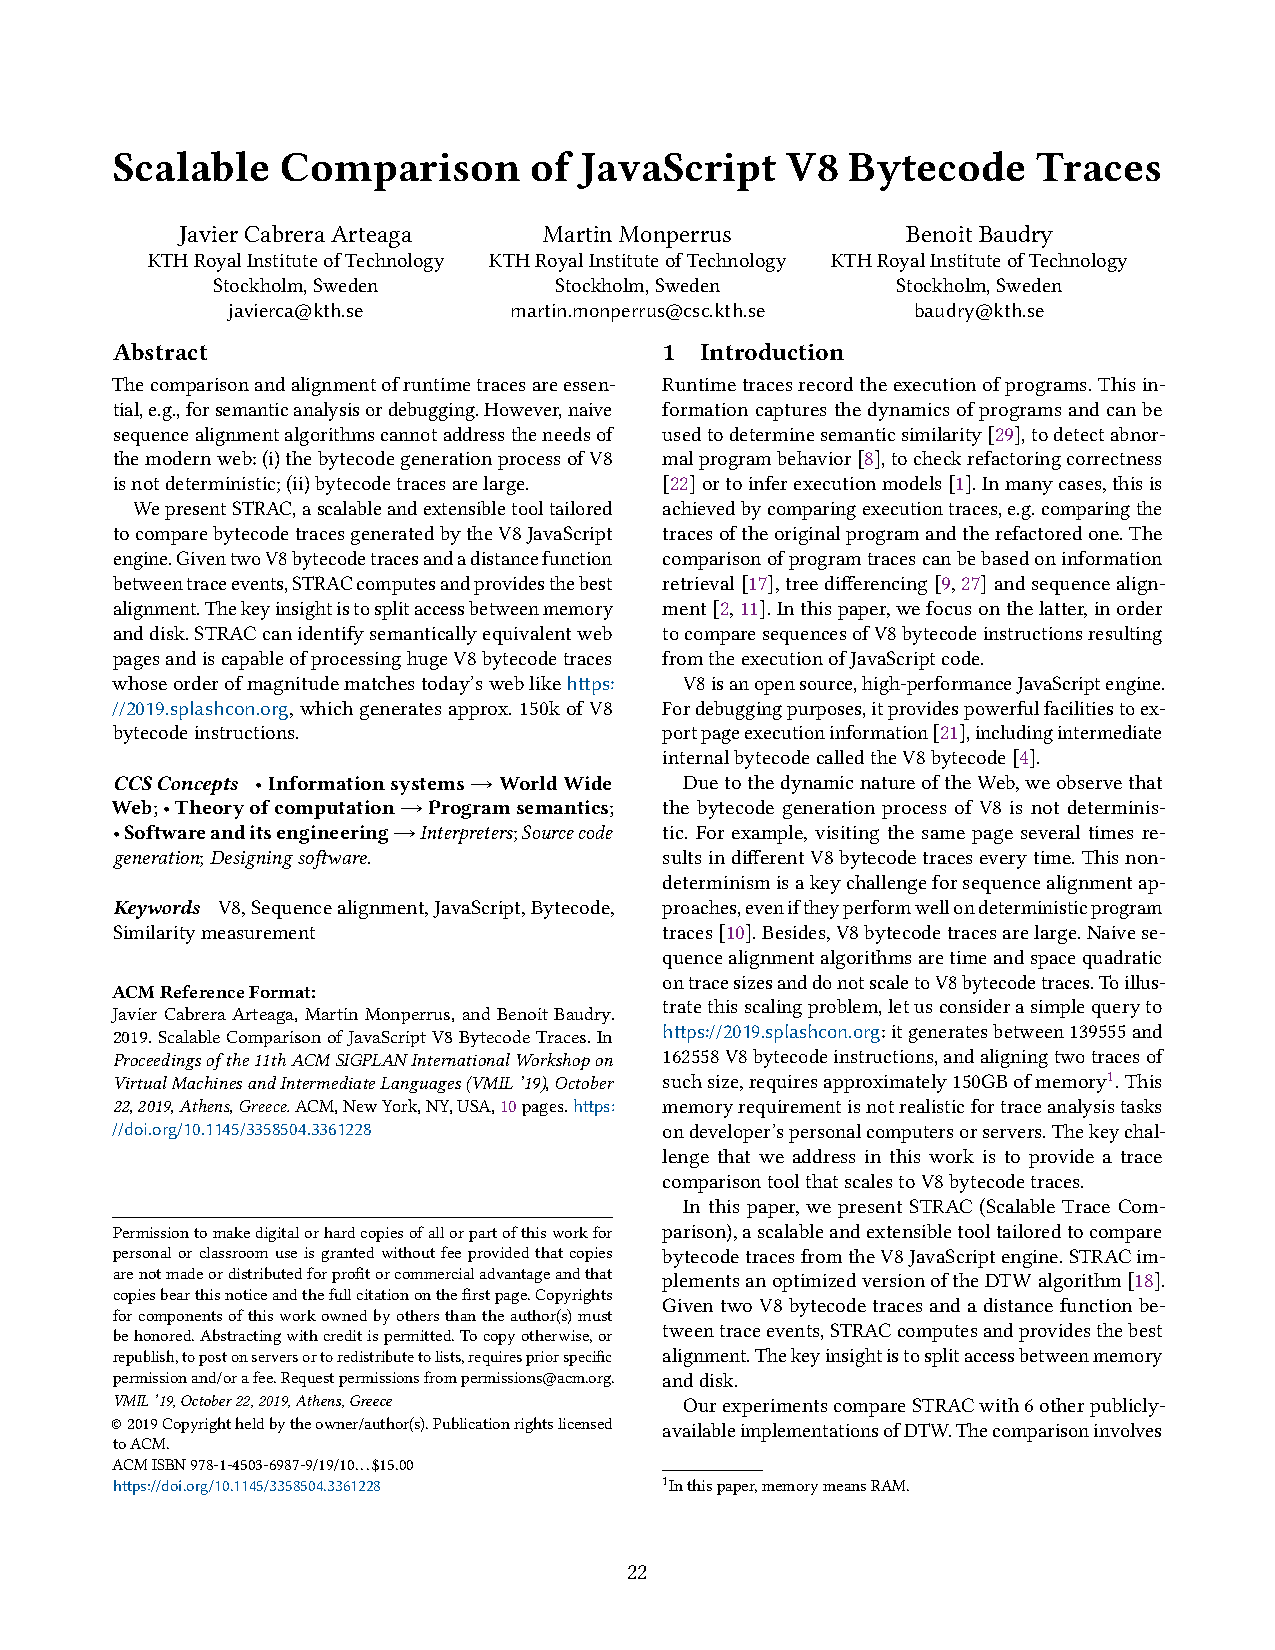
\includepdf[pages=1-10]{papers/STRAC.pdf}} %
    {} %
    
\printindex

\end{document}
\endinput
%%
%% End of file `kth-demo.tex'.
